\documentclass{standalone}
\usepackage{tikz}
\usepackage{float}
\usepackage{lmodern}
\usepackage{amsmath}
\usepackage{xcolor}
\usetikzlibrary{calc}
\usetikzlibrary{intersections}
\usetikzlibrary{decorations.markings, decorations.pathreplacing}

\begin{document}

\centering

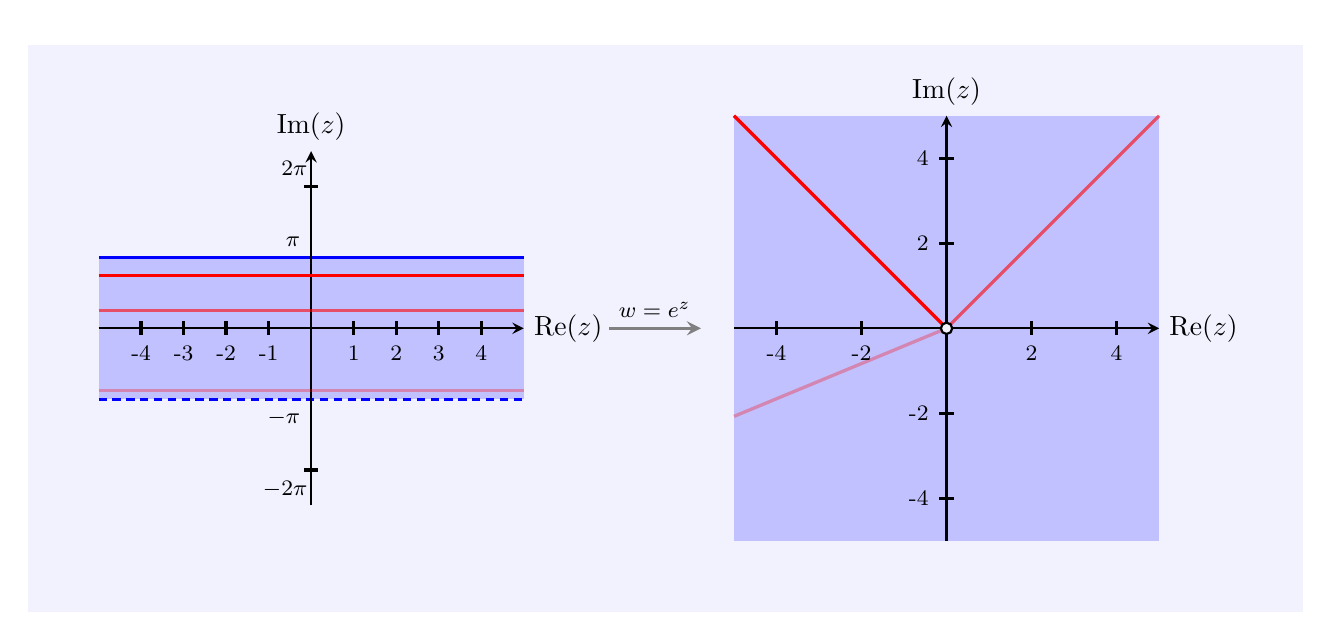
\begin{tikzpicture}[scale=0.9]
% conversion from cm to pt and vice versa
\pgfmathsetmacro{\CmToPt}{28.3464566929}
\pgfmathsetmacro{\PtToCm}{0.0352777778}
% define styles used in this picture
\tikzset{
BigTextFont/.style={font=\normalsize},              % Big text font
every node/.style={font=\footnotesize,text=black},  % Small text font
every path/.style={very thick},
arrowstyle/.style={->, >=stealth}}

\colorlet{BlueBackground}{blue!5}
% Background for entire canvas
\fill[BlueBackground] (-4.0,-4.0) rectangle (14.0,4.0);

% custom colors
\definecolor{ContourHighlight}{rgb}{255,0,0}        % color to highlight contours of the function
\definecolor{BlueDomain}{rgb}{0, 0, 128}

% control dimensions of filled area in domain of function
\pgfmathsetmacro{\AreaHeight}{1.0}
\pgfmathsetmacro{\AreaWidth}{3.0}

% draw the filled area and its borders
\fill[color=BlueDomain, opacity=0.2] (-\AreaWidth, -\AreaHeight) -- (\AreaWidth, -\AreaHeight) -- (\AreaWidth, \AreaHeight) -- (-\AreaWidth, \AreaHeight) -- cycle;
\draw[color=BlueDomain, densely dashed] (-\AreaWidth, -\AreaHeight) -- (\AreaWidth, -\AreaHeight);
\draw[color=BlueDomain] (\AreaWidth, \AreaHeight) -- (-\AreaWidth, \AreaHeight);

%% AXES
% function for drawing axes complex plane
\newcommand{\DrawComplexAxes}[2]{%
  \pgfmathsetmacro{\AxisSizeX}{#1}
  \pgfmathsetmacro{\AxisSizeY}{#2}
  \draw[arrowstyle, thick]  (-\AxisSizeX/2, 0) -- (\AxisSizeX/2, 0) node[pos=1, right, BigTextFont] {$\mathrm{Re}(z)$};
  \draw[arrowstyle, thick] (0, -\AxisSizeY/2) -- (0, \AxisSizeY/2) node[pos=1, above, BigTextFont] {$\mathrm{Im}(z)$};
}

\DrawComplexAxes{\AreaWidth * 2}{\AreaHeight * 5.0}

% ticks on x-axis
\pgfmathsetmacro{\Ticksize}{0.1}
\pgfmathsetmacro{\XTickscaling}{0.6}
\foreach \x in {-4,-3,-2,-1,1,2,3,4} {
\draw (\x * \XTickscaling,\Ticksize) -- (\x * \XTickscaling,-\Ticksize) node[below] {\x};
}

% ticks on y-axis
\pgfmathsetmacro{\YTickscaling}{\AreaHeight}
\node[above left] at (0, 1*\YTickscaling) {$\pi$};
\node[below left] at (0, -1*\YTickscaling) {$-\pi$};
\draw (-\Ticksize, 2*\YTickscaling) -- (\Ticksize, 2*\YTickscaling) node[above left] {$2 \pi$};
\draw (-\Ticksize, -2*\YTickscaling) -- (\Ticksize, -2*\YTickscaling) node[below left] {$-2 \pi$};



%% FUNCTION CONTOURS
% macro for drawing horitzontal line in domain of function
\newcommand{\DrawHorizontalLine}[2]{% #1 = x-value, #2 = opacity
  \pgfmathsetmacro{\YVal}{#1 / (pi)}
  \pgfmathsetmacro{\Opac}{#2}
  \draw[color=ContourHighlight, opacity=\Opac]
    (-\AreaWidth, \YVal*\YTickscaling) --
    (\AreaWidth, \YVal*\YTickscaling);
}

% define scaling in range of function
\pgfmathsetmacro{\SecondPlotScale}{0.6}

\pgfmathsetmacro{\BackgroundSize}{\AreaWidth*1.0}

% macro for drawing circle in range of function
\newcommand{\DrawRayToSquare}[2]{%
  \pgfmathsetmacro{\Angle}{#1 * 180/pi}
  \pgfmathsetmacro{\Opac}{#2}
  % Define square path as a closed shape (for intersection)
  \path[name path=FunctionRange] (-\BackgroundSize, -\BackgroundSize) rectangle (\BackgroundSize, \BackgroundSize);

  % Define ray path from origin at given angle (in degrees)
  \path[name path=ray] (0,0) -- ++({cos(\Angle)*2*\BackgroundSize}, {sin(\Angle)*2*\BackgroundSize});

  % Compute intersection point
  \path[name intersections={of=ray and FunctionRange, name=i}];

  % Draw ray from center to intersection
  \draw[color=ContourHighlight, opacity=\Opac] (0,0) -- (i-1);
}



% define x-values vertical lines
\pgfmathsetmacro{\XOne}{-pi * 7/8}
\pgfmathsetmacro{\XTwo}{pi / 4}
\pgfmathsetmacro{\XThree}{pi * 3/4}

% draw vertical lines
\DrawHorizontalLine{\XOne}{0.3}
\DrawHorizontalLine{\XTwo}{0.6}
\DrawHorizontalLine{\XThree}{1.0}

% 2nd plot: contours in the range of the function
\begin{scope}[xshift = \AreaWidth * 3 * \CmToPt]
  % background for subcanvas 
  \pgfmathsetmacro{\BackgroundSize}{\AreaWidth*1.0}
  \fill[color=BlueDomain, opacity=0.2] (-\BackgroundSize, -\BackgroundSize) rectangle (\BackgroundSize, \BackgroundSize);
  % draw axes
  \DrawComplexAxes{\AreaWidth * 2}{\AreaWidth * 2}
  % contour from the function
  \DrawRayToSquare{\XOne}{0.3}
  \DrawRayToSquare{\XTwo}{0.6}
  \DrawRayToSquare{\XThree}{1.0}
  
  % draw ticks on the axes
  % ticks on x- and y-axes
  \pgfmathsetmacro{\Ticksize}{0.1}
  \foreach \index in {-4,-2,2,4} {
  \draw (\index * \SecondPlotScale,\Ticksize) -- (\index * \SecondPlotScale,-\Ticksize) node[below] {\index};
  \draw (\Ticksize, \index * \SecondPlotScale) -- (-\Ticksize, \index * \SecondPlotScale) node[left] {\index};
  }

  % draw small circle to indicate that 0 is not part of the range of the function
  \draw[fill=BlueBackground, draw=black, thick] (0,0) circle [radius=0.08];
\end{scope}

% arrow for the function
\draw[arrowstyle, color=gray, postaction={decorate}, 
    decoration={markings, mark=at position 0.5 with {\node[above] {$w = e^{z}$};}}]
     (\AreaWidth + 1.2, 0.0) -- (2*\AreaWidth - 0.5, 0.0);

\end{tikzpicture}

\end{document}